\documentclass[11pt,a4paper]{article}
\usepackage[T1]{fontenc}
\usepackage[utf8]{inputenc}
\usepackage{lmodern,microtype}
\usepackage[margin=25mm,headheight=15pt]{geometry}
\usepackage{amsmath,amssymb,amsthm,mathtools,bm,mathrsfs}
\usepackage{booktabs,longtable,array,enumitem,needspace}
\usepackage{graphicx,xcolor,tikz}
\usetikzlibrary{arrows.meta,positioning}
\usepackage{csquotes}
\usepackage[backend=biber,style=numeric,sorting=none,maxbibnames=20,giveninits=true,doi=true,url=false,isbn=false]{biblatex}
\addbibresource{references.bib}
\usepackage[colorlinks=true,linkcolor=blue!45!black,citecolor=blue!45!black,urlcolor=blue!55!black]{hyperref}
\usepackage[nameinlink,noabbrev]{cleveref}
\usepackage{fancyhdr}
\pagestyle{fancy}
\fancyhf{}
\fancyhead[L]{\small Acoustic Freeform Lab}
\fancyhead[R]{\small Theoretical formulation}
\fancyfoot[C]{\thepage}
\setlength{\parskip}{0.35em}
\setlength{\parindent}{1.2em}
\setlist{itemsep=0.2em,topsep=0.3em}
\numberwithin{equation}{section}
\newtheorem{proposition}{Proposition}[section]
\newtheorem{remark}[proposition]{Remark}
\newcommand{\dd}{\,\mathrm d}
\newcommand{\R}{\mathbb R}
\newcommand{\C}{\mathbb C}
\newcommand{\nn}{\bm n}
\newcommand{\Id}{\bm I}
\newcommand{\Pg}{\bm P_\Gamma}
\newcommand{\Gs}{\nabla_\Gamma}
\newcommand{\jump}[1]{\left[\!\left[#1\right]\!\right]}
\newcommand{\norm}[1]{\left\lVert#1\right\rVert}
\newcommand{\inner}[2]{\left\langle#1,#2\right\rangle}
\DeclareMathOperator{\tr}{tr}
\DeclareMathOperator{\rank}{rank}
\DeclareMathOperator{\diag}{diag}
\DeclareMathOperator{\Rea}{Re}
\DeclareMathOperator{\Ima}{Im}
\DeclareMathOperator*{\argmin}{arg\,min}
\hypersetup{pdftitle={Acoustic formation and stabilization of Cartesian optical interfaces},pdfauthor={Acoustic Freeform Lab},pdfsubject={General theoretical formulation of acoustic inverse design for stigmatic liquid diopters}}
\title{Acoustic formation and stabilization of Cartesian optical interfaces\\[0.5em]
\large A general formulation of optical targets, wave--fluid coupling, inverse design and control}
\author{Acoustic Freeform Lab\\\small Private research manuscript}
\date{6 September 2026 \quad---\quad Version 1.0}
\begin{document}
\maketitle
\begin{abstract}
This manuscript formulates the creation of optical liquid interfaces by acoustic
actuation without prescribing a chamber, emitter arrangement, fluid pair or
operating frequency. The principal targets are Cartesian surfaces that image one
axial point stigmatically into another; more general aspherical targets enter the
same mechanical problem. We distinguish transient formation, stable driven
operation and persistence after actuation ends. A continuum model provides the
reference description, while a conditional separation of acoustic and interface
timescales yields explicit radiation-traction and actuator-response equations.
The required static traction is derived by constrained variation of capillary and
gravitational energy. The acoustic inverse problem is expressed through Hermitian
quadratic forms, with feasibility conditions and a semidefinite relaxation whose
physical interpretation depends on coherence. Implicit sensitivities, adjoint
equations and constrained optimal-control conditions connect surface accuracy,
formation trajectories and stability. A conditional obstruction shows why a
finite acoustic pulse cannot permanently retain a non-equilibrium shape in a
fully relaxed, unchanged liquid. All statements of feasibility and stability are
conditional on specified material laws and boundary data. No numerical design,
simulation result, or universal controllability claim is made.
\end{abstract}
\tableofcontents
\newpage
\section{Problem, scope and conventions}\label{sec:scope}

The design question is the following: given a smooth target interface inside a
cylinder, which admissible acoustic source distributions can form it and
maintain it with specified accuracy and stability? The target is initially an
arbitrary surface. Its compatibility with the fluid volume and boundaries,
the required stress, the range of realizable acoustic loads, and its dynamic
stability are separate conditions. Cartesian optical surfaces enter only after
these general conditions have been formulated.

Existing observations establish deformation by radiation pressure and the
importance of the interaction between the wave and its evolving interface
\cite{bertin2012,chesneau2022}. Time-dependent deformations have also been
measured under localized ultrasound \cite{sisombat2023}. These results motivate
the present formulation, but do not establish arbitrary surface controllability
or optical precision for an unspecified apparatus.

\subsection{Cylindrical geometry and data left as arguments}
Let $t$ denote physical time, and let $T_f>0$ denote a chosen formation horizon.
The position vector is $\bm x=(x_1,x_2,z)\in\R^3$. Define a reference cylinder
of radius $R_c>0$ and height $H_c=z_t-z_b>0$ by
\begin{equation}
 \mathcal D_c=\{\bm x:x_1^2+x_2^2<R_c^2,\ z_b<z<z_t\}.
 \label{eq:cylinder}
\end{equation}
Here $z_b$ and $z_t$ are the bottom and top coordinates. The cylinder fixes
the container geometry, not a symmetry of the state. An interface, source
field or perturbation may depend on all three coordinates. A connected fluid region
$\Omega^-(t)$ is surrounded, at least across its optical interface, by a second
fluid region $\Omega^+(t)$. The superscript $-$ labels the lens material and $+$
the adjoining fluid; either may be the incident optical medium. A gas is
included as a possible adjoining fluid, without replacing it by a vacuum or a
pressure-release boundary at this stage.

Let $\Gamma(t)$ be the deformable fluid--fluid interface and
$\Gamma_{\rm opt}(t)\subseteq\Gamma(t)$ its clear optical part. Other boundaries
may support the liquid, radiate acoustic energy, or couple to elastic solids.
The actuator boundary, when actuation is imposed on a boundary, is denoted by
$\Gamma_a$. The contact line, when one exists, is
$\mathcal C(t)=\partial\Gamma(t)$ on a supporting solid. The two phases
partition the fluid-filled part of the cylinder; additional immersed bodies
require their geometry and boundary conditions as explicit data. Closed free
interfaces have no contact line. A graph over a circular disk is one admissible
representation, not a requirement; overhangs need a general surface description.

When acoustic motion is prescribed on a wall, $\partial\mathcal D_c$ is its
reference or cycle-mean position. The full waveform problem uses the moving
wall, and its linearization transfers the condition to that reference surface.
An exactly fixed impermeable wall cannot also have a nonzero normal velocity.
Any open boundary or volume source must declare its mass and energy exchange.

The unit normal $\nn$ points from $\Omega^-$ to $\Omega^+$. Define the identity
tensor $\Id$, tangential projector $\Pg=\Id-\nn\otimes\nn$, surface gradient
$\Gs=\Pg\nabla$, and signed total curvature
$\kappa=\Gs\cdot\nn$. Thus a spherical lens-fluid region has positive
curvature. The symbol $\otimes$ denotes a tensor product. For a quantity with
two interface traces, define its jump as
$\jump{f}=f^+-f^-$. These choices fix the signs of all interfacial forces.

The supplied physical data must include the fluid constitutive laws,
body force, external boundaries, wetting law or pinning
constraint, conserved fluid masses, actuator response and admissible command
set. A device-independent formulation leaves those data as arguments of the
problem; it cannot eliminate their influence on the answer. In particular,
optical conjugates alone cannot determine electrical voltages. No particular
aperture, fill height, immersion fluid, source count or operating frequency is
assigned. Arbitrary sources means arbitrary functions within a declared
physical admissible set, not independent prescription of pressure and velocity
at every interface point.

\subsection{Three meanings of a stable optical result}
Let $\Gamma_\star$ denote a desired interface. We distinguish:
\begin{enumerate}
\item \emph{Transient formation}: the trajectory approaches $\Gamma_\star$
within a finite time, possibly with nonzero fluid velocity or acoustic energy.
\item \emph{Driven operation}: constant, periodic, or feedback-controlled
actuation maintains acceptable optics and rejects specified disturbances.
\item \emph{Unforced retention}: the shape remains acceptable after the sound,
associated flows, and thermal transients have decayed.
\end{enumerate}
A pulse means actuation of finite temporal support, with a specified waveform
and bandwidth. It does not imply an ideal Dirac impulse. A periodically repeated
pulse train is continued actuation. Solidification is a change of constitutive
law and belongs to a distinct retention problem.

\begin{figure}[htbp]
\centering
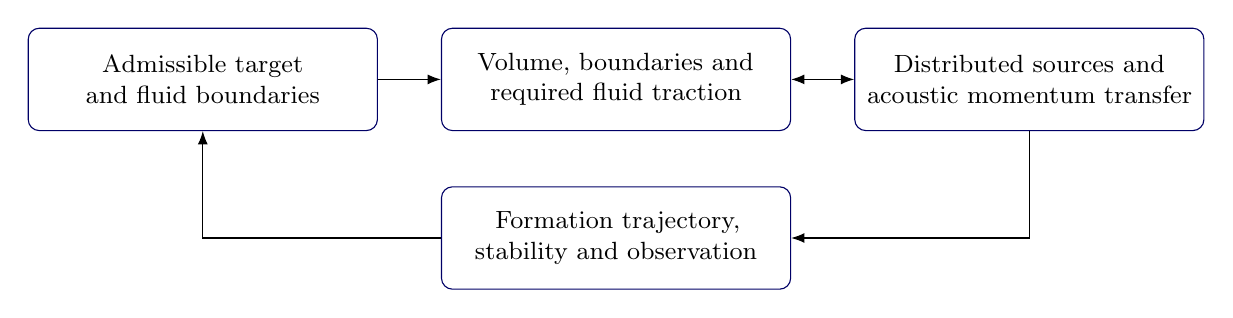
\begin{tikzpicture}[>=Latex,node distance=7mm and 8mm,
 box/.style={draw=blue!40!black,rounded corners,align=center,
 text width=42mm,minimum height=13mm,font=\small}]
 \node[box] (opt) {Admissible target\ and fluid boundaries};
 \node[box,right=of opt] (mech) {Volume, boundaries and\ required fluid traction};
 \node[box,right=of mech] (wave) {Distributed sources and\ acoustic momentum transfer};
 \node[box,below=of mech] (dyn) {Formation trajectory,\ stability and observation};
 \draw[->] (opt)--(mech);
 \draw[<->] (mech)--(wave);
 \draw[->] (wave.south)|-(dyn.east);
 \draw[->] (dyn.west)-|(opt.south);
\end{tikzpicture}
\caption{Dependencies of the inverse problem. Changes of shape alter the acoustic
field; optical performance must be assessed along the resulting physical state.}
\label{fig:dependencies}
\end{figure}

\subsection{Model hierarchy and mathematical status}
The reference continuum description assumes immiscible phases, a regular sharp
interface, and no mass transfer through that interface during shaping. A
Newtonian stress law is supplied explicitly, while non-Newtonian rheology,
solidification, cavitation and topology changes require additional equations.
These are physical modeling choices, not assumptions about a particular
container. Three conditional reductions are identified where used:
\begin{enumerate}[label=(\roman*)]
\item geometric optics in homogeneous isotropic optical media;
\item small acoustic perturbations with a justified averaging timescale;
\item quiescent, constant-density, constant-surface-tension equilibria for an
explicit shape-to-traction formula.
\end{enumerate}
The dynamic formulation retains fluid inertia. Creeping flow appears only as an
explicit limiting case. A stationary interface may coexist with streaming;
such a state requires a steady-flow solve and is not a quiescent equilibrium.

Derivatives below are conditional on a regular local solution and differentiable
state and geometry maps. Smooth interface patches are taken at least $C^3$ for
the displayed curvature variations. We neither prove global well-posedness of
the moving-interface problem nor assert existence of a solution for every
target. Propositions are stated with the assumptions needed for their proofs.
The optimization objectives and design workflow are a proposed synthesis of
these equations. Explicit weak forms, source adjoints and conditional proofs
are given for identified subproblems; the full thermoviscous moving-interface
system is a reference formulation, not a proved globally solvable inverse.
Numerical continuation is neither an assumption nor a step required by the
inverse equations. Numerical experiments will test this formulation.

\subsection{Notation used throughout}
The table defines the principal quantities before their subsequent use. More
specialized symbols are introduced immediately before their equations. All
physical lengths, times and stresses use SI units unless nondimensionalization
is stated.
\begin{longtable}{@{}p{29mm}p{112mm}@{}}
\toprule Symbol & Meaning and units \\\midrule\endhead
$\rho_\ell,\bm v_\ell,p_\ell$ & Instantaneous density, velocity and pressure in
phase $\ell\in\{-,+\}$; $\mathrm{kg\,m^{-3}}$, $\mathrm{m\,s^{-1}}$, $\mathrm{Pa}$.\\
$\bm T_\ell,\bm\tau_\ell$ & Total Cauchy stress and viscous stress; $\mathrm{Pa}$.\\
$\mu_\ell,\zeta_\ell$ & Shear and bulk viscosities; $\mathrm{Pa\,s}$.\\
$\Theta_\ell,e_\ell,k_\ell$ & Temperature, specific internal energy and thermal
conductivity; $\mathrm K$, $\mathrm{J\,kg^{-1}}$, $\mathrm{W\,m^{-1}\,K^{-1}}$.\\
$\sigma,\Phi$ & Surface tension and conservative body-force potential per unit
mass; $\mathrm{N\,m^{-1}}$, $\mathrm{m^2\,s^{-2}}$. The body acceleration is $-\nabla\Phi$.\\
$\lambda_V$ & Pressure multiplier imposing lens volume in an incompressible
reduction; $\mathrm{Pa}$.\\
$\bm U_\ell,p^h_\ell$ & Slow hydrodynamic velocity and pressure in an averaged
description; $\mathrm{m\,s^{-1}}$, $\mathrm{Pa}$.\\
$P_\ell,\bm V_\ell$ & Complex peak acoustic pressure and velocity amplitudes;
$\mathrm{Pa}$ and $\mathrm{m\,s^{-1}}$. They are distinct from the slow fields.\\
$\bm R_\ell,\bm t_{\rm ac},\Pi$ & Acoustic momentum-flux tensor, effective
interfacial acoustic traction, and its outward normal component; $\mathrm{Pa}$.\\
$n_o,n_i,\lambda_{\rm opt}$ & Incident and transmitted optical indices
(dimensionless), and vacuum optical wavelength ($\mathrm m$).\\
$\bm O,\bm I$ & Object and image points; the object subscript is the letter $o$.\\
$\eta,\bm w$ & Normal surface displacement ($\mathrm m$) and complex peak
mechanical emitter velocities ($\mathrm{m\,s^{-1}}$ per component).\\
$\bm a,\bm y$ & General actuator command field and full physical state; each
may be an infinite-dimensional collection of fields. Units depend on the
declared actuator and constitutive model.\\
\bottomrule
\end{longtable}
Bold symbols denote vectors or tensors. The dagger $\dagger$ denotes conjugate
transpose, the superscript $T$ ordinary transpose, and an asterisk complex
conjugation. Inner products are real duality pairings unless explicitly complex;
$\Rea$ and $\Ima$ denote real and imaginary parts.

\section{Cartesian targets and optical measures}\label{sec:optics}

\subsection{An unsquared optical-path construction}
Fix a vacuum wavelength $\lambda_{\rm opt}$, positive unequal homogeneous indices
$n_o,n_i$, and distinct conjugate points $\bm O,\bm I$. The signs $s_o,s_i$ are
$+1$ for a real object or real image, respectively, and $-1$ for a virtual one.
For an interface point $\bm x$ distinct from both foci, let
$R_o=|\bm x-\bm O|$ and $R_i=|\bm x-\bm I|$. Define the signed optical path
$\Psi$ and a constant path level $C$ by
\begin{equation}
 \Psi(\bm x)=s_o n_oR_o+s_i n_iR_i,\qquad
 \Gamma_{\rm opt,\star}\subset\{\bm x:\Psi(\bm x)=C\}.
 \label{eq:cartesian-implicit}
\end{equation}
Both $\Psi$ and $C$ have units of length. The constant is fixed by a chosen
vertex or by compatible mounting and volume data. For two real conjugates this
is the usual weighted sum of distances. Signed paths extend the construction to
virtual conjugates. The formulas and Cartesian-surface classification follow
Silva-Lora and Torres \cite{silva2020}; the mechanical and control formulation
below is separate from that paper's two-surface singlet construction.

Let $\bm d_o=s_o(\bm x-\bm O)/R_o$ be the incident propagation direction and
$\bm d_i=s_i(\bm I-\bm x)/R_i$ the desired transmitted direction. Then
\begin{equation}
 \nabla\Psi=n_o\bm d_o-n_i\bm d_i,\qquad
 \Gs\Psi=0\ \Longrightarrow\ n_o\Pg\bm d_o=n_i\Pg\bm d_i.
 \label{eq:fermat-snell}
\end{equation}
This directly supplies the tangential Snell condition. Squaring
\cref{eq:cartesian-implicit} gives a quartic, but can add branches; its real
roots alone do not certify the intended refracting surface.

To select transmission, let $\bm m$ be the unit surface normal pointing from the
incident medium into the transmitted medium. Thus $\bm m=\pm\nn$ depending on
which fluid light enters first. Set $c_o=\bm d_o\cdot\bm m$ and
$\eta_n=n_o/n_i$. The physically transmitted unit direction $\bm d_t$ is
\begin{equation}
 \bm d_t=\eta_n\bm d_o+
 \left[\sqrt{1-\eta_n^2(1-c_o^2)}-\eta_n c_o\right]\bm m.
 \label{eq:snell-vector}
\end{equation}
The branch must satisfy $c_o>0$, a nonnegative square-root argument,
$\bm d_t\cdot\bm m>0$, and $\bm d_t=\bm d_i$ throughout the admitted aperture.
These exclude back-facing and totally internally reflecting branches. A finite
distance from grazing transmission is also needed for well-conditioned optical
sensitivities.

\subsection{The four axial conjugate parameters}
Choose the vertex as the origin, with optical propagation there in the positive
$z$ direction. Let $z_o,z_i$ be the signed axial coordinates of the conjugates,
and define cylindrical radius $r=\sqrt{x^2+y^2}$. For finite nonzero conjugates,
$s_o=-\operatorname{sgn}(z_o)$ and $s_i=\operatorname{sgn}(z_i)$. The level fixed
by the vertex is $C=-n_oz_o+n_iz_i$. In particular, for $z_o<0<z_i$,
\begin{equation}
 n_o\sqrt{r^2+(z-z_o)^2}+n_i\sqrt{r^2+(z_i-z)^2}
 =-n_oz_o+n_iz_i.
 \label{eq:real-cartesian}
\end{equation}

For the paper's parametric representation, define inverse lengths
$a=1/z_o$, $b=1/z_i$, and $D=n_i a-n_o b$. When the denominators are nonzero,
define the form parameters $\mathsf O$ (inverse length), $\mathsf G$
(dimensionless), $\mathsf T$ (inverse length cubed), and $\mathsf S$ (inverse
length squared) as
\begin{align}
 \mathsf O&=\frac{n_i b-n_o a}{n_i-n_o}, &
 \mathsf G&=\frac{(n_i^2a-n_o^2b)^2}{n_i n_o D(n_i b-n_o a)},\label{eq:gots-a}\\
 \mathsf T&=\frac{(n_i-n_o)(n_i+n_o)^2a^2b^2}{4n_i n_oD}, &
 \mathsf S&=\frac{(n_i+n_o)(n_i^2a-n_o^2b)ab}{2n_i n_oD}.
 \label{eq:gots-b}
\end{align}
The signed vertex graph curvature is $z''(0)=\mathsf O$; it is not the total
mechanical curvature $\kappa$. For an upward physical normal at an axisymmetric
vertex, $\kappa(0)=-2\mathsf O$.

Define the polar distance $\varrho=\sqrt{r^2+z^2}$, which is \emph{not} the
cylindrical radius $r$ or either fluid density. The parameters satisfy
$\mathsf S^2=\mathsf O\mathsf G\mathsf T$. The Cartesian polynomial in these
coordinates is
\begin{equation}
 \mathsf O\mathsf Gz^2-2(1+\mathsf S\varrho^2)z
       +(\mathsf O+\mathsf T\varrho^2)\varrho^2=0.
 \label{eq:gots-polynomial}
\end{equation}
Solving this quadratic in $z$, selecting the branch through the vertex, and
rationalizing yields
\begin{equation}
 z(\varrho)=
 \frac{(\mathsf O+\mathsf T\varrho^2)\varrho^2}
 {1+\mathsf S\varrho^2+
   \sqrt{1+(2\mathsf S-\mathsf O^2\mathsf G)\varrho^2}},\qquad
 r(\varrho)=\sqrt{\varrho^2-z(\varrho)^2}.
 \label{eq:gots-parametric}
\end{equation}
The unsquared path and transmission tests remain necessary. Singular GOTS
coordinates need not imply a singular physical surface; in that event use
\cref{eq:cartesian-implicit} directly. Equal indices, coincident foci, and
degenerate conjugates require their own optical interpretation rather than
division by a vanishing coefficient.

For collimated incidence, take $z_o\to-\infty$ and subtract the divergent constant
path. The finite condition for a real image is
$n_oz+n_i(\sqrt{r^2+(z_i-z)^2}-z_i)=0$. Here $\mathsf S=\mathsf T=0$ and the
conic constant $K=-(n_o/n_i)^2$. Writing the signed vertex curvature as
$c_v=n_i/[z_i(n_i-n_o)]$ gives
\begin{equation}
 z(r)=\frac{c_v r^2}{1+\sqrt{1-(1+K)c_v^2r^2}}.
 \label{eq:collimated-conic}
\end{equation}
For finite conjugates, a Cartesian surface is generally not an exact conic, and
$\mathsf G$ must not be identified with a fitted conic constant.

\subsection{Geometric compatibility and limits of arbitrariness}
For fixed homogeneous indices and two fixed points, $\Psi$ is invariant under
rotation about their joining axis. Consequently a regular connected Cartesian
level surface belongs to a surface of revolution. An arbitrary non-axisymmetric
surface is generally incompatible with exact single-interface point-to-point
stigmatism under these optical assumptions. Arbitrary aspheres remain valid
mechanical targets, but require a correspondingly different optical objective
or incident wavefront.

More generally, let $S_o(\bm x)$ and $S_i(\bm x)$ be incident and desired
transmitted eikonal functions, measured as optical path lengths. In homogeneous
media they satisfy $|\nabla S_o|=n_o$ and $|\nabla S_i|=n_i$, with gradients
pointing along propagation. A purely refracting interface with no imposed
phase discontinuity must lie on $S_o-S_i=C$. The point-conjugate choice is
$S_o=s_on_oR_o$, $S_i=-s_in_iR_i$, recovering
\cref{eq:cartesian-implicit}. A non-axisymmetric target can thus be coupled to
a specified different wavefront-design problem, but the necessary incident
wavefront must be physically supplied rather than assumed to arise from the
same two point conjugates.

The target must also be compatible with the available fluid mass, supporting
boundaries and allowed contact-line motion. In an incompressible model, fixing
the entire interface and its other boundaries fixes the enclosed volume. A
single optical path constant cannot generally enforce an arbitrary boundary
curve and an independently prescribed volume. Possible design freedoms are a
non-optical annulus, a movable support, a reservoir, or revised conjugates; none
is silently introduced here.

The incident directions in \cref{eq:fermat-snell} are specified in a homogeneous
incident medium. If light first crosses a window or another liquid surface,
that preceding optical system must produce those directions and optical paths.
Similarly, solidifying a liquid can change its index and shape. A liquid
Cartesian diopter is therefore not automatically a Cartesian finished lens.
Exact axial stigmatism at one wavelength does not establish the Abbe sine
condition, off-axis aplanatism, or achromatism.

\subsection{Optical objectives and a slope-sensitive identity}
Let $\mathcal P$ be a two-dimensional entrance pupil, $\bm\xi\in\mathcal P$ its
ray label, and $\bm X_\Gamma(\bm\xi)$ the ray's first intended intersection with
the interface. Every admitted ray must reach the intended transmitting patch
and have an unobstructed optical continuation. Let $\mathrm d\mu(\bm\xi)$ be a nonnegative normalized measure
representing the selected illumination, so $\int_{\mathcal P}\mathrm d\mu=1$.
Define the mean signed path $\overline\Psi=\int_{\mathcal P}
\Psi(\bm X_\Gamma)\mathrm d\mu$ and path departure
$W=\Psi(\bm X_\Gamma)-\overline\Psi$. Choose a positive optical-path tolerance
$W_{\rm ref}$ with units of length and an angular tolerance
$\theta_{\rm ref}>0$ in radians. Two dimensionless objectives are
\begin{equation}
 J_W=\int_{\mathcal P}\frac{W^2}{W_{\rm ref}^2}\mathrm d\mu,
 \qquad
 J_d=\int_{\mathcal P}
 \frac{\norm{\Pg(\bm d_t-\bm d_i)}^2}{\theta_{\rm ref}^2}\mathrm d\mu.
 \label{eq:optical-objectives}
\end{equation}
The projector and directions are evaluated at $\bm X_\Gamma$. Removing
$\overline\Psi$ removes an optically irrelevant piston; it does not move either
conjugate. A specified geometric target may additionally fix $C$ and the vertex.

For any physically transmitted surface, tangential Snell refraction gives the
exact identity
\begin{equation}
 n_i\Pg(\bm d_t-\bm d_i)=\Gs\Psi.
 \label{eq:opd-slope-identity}
\end{equation}
Thus a small mean-square path error alone does not control ray error: a small
amplitude but rapidly varying path departure can have a large surface gradient.
Using $J_d$, or an equivalent derivative-sensitive optical objective, prevents
accepting such a surface solely on its path variance. Near grazing transmission,
even small tangential direction errors can produce large changes in the normal
component; the non-grazing condition must therefore be retained.

For a real image, define a detector plane through $\bm I$ with unit normal
$\bm e_i$, and require $\bm d_t\cdot\bm e_i>0$. Its ray intersection is
$\bm Y=\bm X_\Gamma+[(\bm I-\bm X_\Gamma)\cdot\bm e_i]
\bm d_t/(\bm d_t\cdot\bm e_i)$, with a positive propagation distance to that
plane. For a prescribed positive spot-radius tolerance
$r_{\rm ref}$, an additional dimensionless cost is
\begin{equation}
 J_{\rm spot}=\int_{\mathcal P}
       \frac{|\bm Y-\bm I|^2}{r_{\rm ref}^2}\mathrm d\mu.
 \label{eq:spot-cost}
\end{equation}
This keeps the requested image fixed. Geometric ray errors are distinct from
the diffraction point-spread function and from measured optical quality.

\input{sections/03_mechanics}
\section{Acoustic transfer, radiation traction and temporal memory}\label{sec:acoustics}

\subsection{When a harmonic reduction is justified}
Let $\omega>0$ be angular carrier frequency, $T_a=2\pi/\omega$ its period,
$T_e$ an envelope variation time, $T_\Gamma$ an interface variation time, and
$\tau_r$ an acoustic energy ring-down time. A fast-time average over an interval
$\Delta t$ requires
\begin{equation}
 T_a\ll\Delta t\ll\min(T_e,T_\Gamma).
 \label{eq:averaging-separation}
\end{equation}
Replacing the field at each instant by a settled harmonic solution also requires
$\tau_r\ll\min(T_e,T_\Gamma)$. A short carrier period alone does not imply
short ring-down in a resonant cavity. When these conditions fail, causal wave
dynamics or the reference continuum equations must be retained.

For a fixed slow state, use the peak-phasor convention
$p_{1\ell}(\bm x,t)=\Rea\{P_\ell(\bm x)e^{-\mathrm i\omega t}\}$ and
$\bm v_{1\ell}(\bm x,t)=\Rea\{\bm V_\ell(\bm x)e^{-\mathrm i\omega t}\}$,
where $\mathrm i^2=-1$ and the subscript $1$ denotes first-order acoustics.
Thus the average of two real harmonic quantities with phasors $A,B$ is
$\frac12\Rea(AB^*)$. For locally homogeneous, inviscid, adiabatic fluids with
negligible mean advection, define the sound speed $c_\ell$ and obtain
\begin{equation}
 -\mathrm i\omega\rho_\ell\bm V_\ell=-\nabla P_\ell,\qquad
 -\mathrm i\omega P_\ell=-\rho_\ell c_\ell^2\nabla\cdot\bm V_\ell,
 \qquad
 \nabla\cdot\left(\frac{\nabla P_\ell}{\rho_\ell}\right)
       +\frac{\omega^2}{\rho_\ell c_\ell^2}P_\ell=0.
 \label{eq:linear-acoustics}
\end{equation}
The sound speed is the isentropic derivative of the equation of state. Loss,
thermal fields and elastic boundaries replace this simple operator when
needed; they are not unspecified tuning coefficients. Boundary-layer
reductions with declared scale conditions are developed in
\cite{bach2018,jorgensen2021}.

The acoustic interface conditions must follow by linearizing the kinematic and
traction conditions on the displaced interface. Let $\Xi$ be its first-order
normal-displacement phasor, in metres. About a quiescent interface,
$\bm V^-\cdot\nn=\bm V^+\cdot\nn=-\mathrm i\omega\Xi$. First-order traction
also contains the capillary curvature variation and the displacement through
base pressure gradients. Neglecting those corrections can yield continuity
of acoustic pressure and normal velocity, as in a common high-frequency
fluid--fluid scattering model \cite{chesneau2022}. That simplification requires
the fast interfacial restoring terms to be small; it is not an exact condition
for capillary waves at all frequencies. A compliant solid or a free surface
requires its own linearized boundary operator.

\subsection{The sign and content of radiation traction}
For the locally homogeneous inviscid acoustic reduction just specified, define
the time-averaged acoustic \emph{momentum flux}
\begin{equation}
 \bm R_\ell=
 \left(\frac{|P_\ell|^2}{4\rho_\ell c_\ell^2}
            -\frac{\rho_\ell|\bm V_\ell|^2}{4}\right)\Id
 +\frac{\rho_\ell}{2}\Rea(\bm V_\ell\otimes\bm V_\ell^*).
 \label{eq:radiation-flux}
\end{equation}
It is minus the radiation-stress convention used in
\cite{chesneau2022}; recording this sign is essential. The effective outward
interfacial traction and its scalar normal component are
\begin{equation}
 \bm t_{\rm ac}=(\bm R_- -\bm R_+)\nn=-\jump{\bm R}\nn,
 \qquad \Pi=\nn\cdot\bm t_{\rm ac}.
 \label{eq:acoustic-traction}
\end{equation}
Let $\bm T^h=-p^h\Id+\bm\tau(\bm U)$ denote slow hydrodynamic stress with the
mean-pressure convention associated with \cref{eq:radiation-flux}. The reduced
interface balance becomes
\begin{equation}
 \jump{\bm T^h}\nn+\bm t_{\rm ac}
       =\sigma\kappa\nn-\Gs\sigma.
 \label{eq:averaged-jump}
\end{equation}
In a consistent bulk momentum balance the acoustic force is
$-\nabla\cdot\bm R$ with the matching mean-pressure definition. A gradient
part can be absorbed into $p^h$; it must not be counted again at the interface.
In thermoviscous or inhomogeneous fluids, the averaged stress, heat source and
boundary-layer forcing have to be derived together from the reference
equations. A scalar normal pressure model does not cover all streaming or
tangential stresses.

Only in a one-sided pressure-release limit, with negligible adjoining-fluid
momentum flux, $P_-\simeq0$ and negligible tangential acoustic velocity at the
surface, does \cref{eq:acoustic-traction} reduce to
\begin{equation}
 \Pi\simeq\frac{\rho_-}{4}|\bm V_-\cdot\nn|^2.
 \label{eq:pressure-release-limit}
\end{equation}
This factor uses peak amplitudes. It must not be transferred unchanged to an
immersed liquid--liquid lens or to a surface supporting appreciable acoustic
pressure. Experiments on liquid interfaces and coupled calculations motivate
retaining the wave--shape interaction, rather than prescribing a load
independent of the deformed geometry \cite{bertin2012,chesneau2022,sisombat2023}.

\subsection{Impulses are causal histories, not instantaneous intensities}
For a fixed geometry and linear acoustics, let $\bm z_a(t)$ collect the wave
state, $\mathcal G_\Gamma(t)$ its causal propagation operator, and
$\mathcal B_\Gamma$ the command-to-source operator. Let $t_0$ be the starting
time and $\bm z_{a,0}$ the initial acoustic state. Then
\begin{equation}
 \bm z_a(t)=\mathcal G_\Gamma(t-t_0)\bm z_{a,0}
       +\int_{t_0}^t\mathcal G_\Gamma(t-s)
                         \mathcal B_\Gamma\bm a(s)\dd s.
 \label{eq:acoustic-memory}
\end{equation}
The radiative load is quadratic in this accumulated field. Two commands with
the same present amplitude can therefore yield different loads because their
histories differ. Changing the interface makes the operator time dependent,
so a fixed convolution kernel is then only a local approximation. Fluid
inertia, viscous relaxation, streaming, temperature and actuator mechanics
provide additional memory variables.

An actual impulse has a restricted mechanical interpretation. Consider a
declared inertial modal reduction with displacement coordinates $\bm q_f$,
modal mass matrix $\mathsf M_f$ and generalized acoustic force
$\bm f_a(t)$. Their component units are metres, kilograms and newtons,
respectively. Let $t_-,t_+$ bracket the effective force pulse, including any
relevant acoustic ring-down. If the shape and $\mathsf M_f$ change negligibly
over that interval and integrated restoring and dissipative forces are small,
integration of momentum gives
\begin{equation}
 \mathsf M_f[\dot{\bm q}_f(t_+)-\dot{\bm q}_f(t_-)]
       \simeq\int_{t_-}^{t_+}\bm f_a(t)\dd t.
 \label{eq:mechanical-impulse}
\end{equation}
The integral has units of momentum. In this limit a short force pulse primarily
changes velocity; the subsequent interface shape follows the inertial,
capillary and viscous evolution. This reduction does not apply when viscous
forces dominate the pulse interval, and an acoustic cycle average still needs
\cref{eq:averaging-separation}. Delivering the correct integrated force is not
the same as arriving at the target with negligible residual motion.

If several carriers $\omega_m$ are used, index $m$ labels their frequencies.
Quadratic products contain cross terms proportional to
$e^{-\mathrm i(\omega_m-\omega_n)t}$. They average away only with appropriate
coherence statistics or an averaging interval satisfying
$|\omega_m-\omega_n|\Delta t\gg1$, together with negligible relevant mechanical
response to the unresolved beats. Nearby carriers can drive slow beat forces;
a sum of independent intensities is not generally their physical load.

\subsection{A mean optical surface is not the entire optical state}
Even when $\Gamma$ denotes a stationary cycle-mean interface, the acoustic
displacement $\xi_a(\bm x,t)=\Rea(\Xi e^{-\mathrm i\omega t})$ can corrugate
its instantaneous position. Let $\delta n_o,\delta n_i$ denote acoustic or
thermal index perturbations along the incident and transmitted ray segments
$\mathcal L_o,\mathcal L_i$. For real conjugates and a nominal stationary
Fermat ray, the first variation of its optical path is
\begin{equation}
 \delta\Psi=(n_o\bm d_o-n_i\bm d_i)\cdot\nn\,\xi_a
       +\int_{\mathcal L_o}\delta n_o\dd s
       +\int_{\mathcal L_i}\delta n_i\dd s.
 \label{eq:fast-optical-error}
\end{equation}
Here $s$ is arclength, and a pupil-constant part is removed to obtain wavefront
error. Virtual conjugates use the corresponding signed path segments.
\Cref{eq:fast-optical-error} is a first-order estimate, not a full
acousto-optic scattering calculation. Material derivatives of optical index,
exposure time, and the fast interface response determine whether these terms
are negligible. A zero-mean wavefront fluctuation can still broaden an
exposure-averaged optical image. The eventual objective must therefore apply
to the intended optical operating state, not only to a plotted mean surface.

\section{From a desired load to emitter commands}\label{sec:inverse}

\subsection{A linear wave response produces a quadratic load}
Fix a geometry, material state and carrier frequency for which the linear wave
problem is well posed. Let $N$ be the number of independent complex mechanical
actuator channels. In one useful boundary representation, let $b_j(\bm x)$ be
the dimensionless normal-velocity pattern of channel $j$ on $\Gamma_a$.
The imposed peak velocity is $\sum_{j=1}^N b_jw_j$. The entries $w_j$ of
$\bm w\in\C^N$ have units of velocity and describe physical motion, not
uncalibrated electrical voltages.

Let $\mathcal A_\Gamma(\omega)$ be the linear wave operator, including all
interface and exterior conditions, and $\mathcal B_\Gamma(\omega)$ the source
operator. Its acoustic state $\bm z_a$ satisfies
\begin{equation}
 \mathcal A_\Gamma(\omega)\bm z_a
       =\mathcal B_\Gamma(\omega)\bm w.
 \label{eq:wave-operator}
\end{equation}
For each phase define a row response $\bm h_{p\ell}(\bm x)$ and a three-row
velocity response $\bm H_{v\ell}(\bm x)$ by
$P_\ell=\bm h_{p\ell}\bm w$ and
$\bm V_\ell=\bm H_{v\ell}\bm w$. The former has units
$\mathrm{Pa\,s\,m^{-1}}$ and the latter is dimensionless. Substitution in
\cref{eq:radiation-flux,eq:acoustic-traction} gives Hermitian matrices
\begin{align}
 \bm K_\ell(\bm x)&=
 \frac{\bm h_{p\ell}^\dagger\bm h_{p\ell}}{4\rho_\ell c_\ell^2}
 -\frac{\rho_\ell}{4}\bm H_{v\ell}^\dagger\bm H_{v\ell}
 +\frac{\rho_\ell}{2}\bm H_{v\ell}^\dagger\nn\nn^T\bm H_{v\ell},\\
 \bm K(\bm x;\Gamma,\omega)&=\bm K_- -\bm K_+,\qquad
 \boxed{\Pi(\bm x)=\bm w^\dagger\bm K(\bm x;\Gamma,\omega)\bm w.}
 \label{eq:quadratic-load}
\end{align}
A Hermitian matrix equals its conjugate transpose, so the load is real.
The matrix $\bm K$ has units $\mathrm{kg\,m^{-3}}$ and need not be positive
semidefinite for two interacting fluids. In the particular limit
\cref{eq:pressure-release-limit}, it is positive semidefinite at each point.
Tangential traction components also have Hermitian quadratic forms.

For a quiescent target, choose $M$ real, dimensionless virtual-displacement
functions $\phi_i$ compatible with the support and satisfying
$\int_\Gamma\phi_i\dd A=0$. Define generalized forces $F_i$, required forces
$b_i$, and integrated matrices $\bm K_i$ by
\begin{equation}
 \bm K_i=\int_\Gamma\phi_i\bm K\dd A,\qquad
 F_i=\bm w^\dagger\bm K_i\bm w,\qquad
 b_i=\int_\Gamma\phi_i(\sigma\kappa+\Delta\rho\Phi)\dd A.
 \label{eq:modal-loads}
\end{equation}
Here $\bm K_i$ has units $\mathrm{kg\,m^{-1}}$, while $F_i,b_i$ are forces.
The target equations are $F_i=b_i$ for all admitted variations. A finite
collection is a necessary projection of the continuum balance; its unsampled
complement and tangential balance still need verification. This construction
is reusable for different targets. The wave response must, however, be updated
when the target changes the scattering geometry.

\subsection{Feasibility, coherence and a useful relaxation}
Define the Hermitian drive matrix $\bm W=\bm w\bm w^\dagger$, whose entries
have units $\mathrm{m^2\,s^{-2}}$. A matrix $\bm W\succeq0$ is positive
semidefinite if $\bm q^\dagger\bm W\bm q\geq0$ for every complex vector
$\bm q$. A nonzero deterministic coherent drive has $\rank\bm W=1$.
Writing $\tr$ for trace, the exact fixed-target problem includes
\begin{equation}
 \tr(\bm K_i\bm W)=b_i,\qquad
 \bm W\succeq0,\quad\rank\bm W\leq1,\qquad
 W_{jj}\leq w_{j,\max}^2.
 \label{eq:lifted-feasibility}
\end{equation}
The positive bounds $w_{j,\max}$ specify peak channel velocities. The rank-zero
case is the undriven state. Let $F_{i,\rm ref}>0$ be meaningful force-error
scales, let $P_{\rm ref}>0$ be a power scale, and let $\beta_P\geq0$ weight
power. If the passive, fixed-geometry actuator model gives average input power
$P_{\rm in}=\bm w^\dagger\bm R_P\bm w$, the Hermitian matrix
$\bm R_P\succeq0$ has units $\mathrm{kg\,s^{-1}}$ and includes the phasor
averaging factor. A practical mismatch objective is
\begin{equation}
 \min_{\bm W}\ \frac12\sum_{i=1}^M
  \left[\frac{\tr(\bm K_i\bm W)-b_i}{F_{i,\rm ref}}\right]^2
       +\beta_P\frac{\tr(\bm R_P\bm W)}{P_{\rm ref}},
 \label{eq:sdr-cost}
\end{equation}
subject to the positivity, rank and hardware constraints. For example, a
pointwise peak pressure bound is linear in $\bm W$:
$\tr(\bm h_p^\dagger\bm h_p\bm W)\leq P_{\max}^2$, where $P_{\max}$ is a
declared pressure limit. Such bounds must hold throughout the specified domain,
not merely at convenient sample points.

Dropping the rank constraint gives a convex semidefinite relaxation when all
other constraints are convex at this fixed geometry. This is a standard
quadratic-optimization construction \cite{luo2010}. Its objective value is a
lower bound for the coherent problem, not proof that a physical coherent
solution attains it. If an optimum has rank one, its factor supplies the drive
up to a global phase. Explicitly, let $\lambda_1>0$ be the single nonzero
eigenvalue and $\bm q_1$ a unit eigenvector of a rank-one optimum. Let $A_j$
and $\varphi_j$ denote channel $j$'s peak velocity and phase, and $v_{a,j}(t)$
its real velocity coefficient. They follow as
\begin{equation}
 \bm w=\sqrt{\lambda_1}\bm q_1,\qquad
 A_j=|w_j|,\quad \varphi_j=\arg w_j,\qquad
 v_{a,j}(t)=A_j\cos(\omega t-\varphi_j).
 \label{eq:drive-recovery}
\end{equation}
The phase of a zero amplitude is immaterial. A higher-rank optimum requires
additional work.

In particular, writing $\bm W$ as a sum of rank-one factors does not create
independent same-frequency coherent fields: those fields add before their
intensity is squared. A higher-rank $\bm W$ can represent a physical covariance
$\mathbb E[\bm w\bm w^\dagger]$ only under an implemented incoherence or
time-multiplexing scheme with appropriate averaging, bandwidth and peak limits.
Covariance bounds constrain second moments; peak limits must additionally hold
for each physically realized waveform.
Switching among patterns must respect the acoustic and mechanical memory in
\cref{sec:acoustics}. Different carrier frequencies generally have different
$\bm K_i(\omega)$ and cannot be substituted into a fixed-frequency factorization
without changing the problem.

\begin{proposition}[A necessary load-feasibility certificate]
Let $\alpha_i$ be real coefficients and suppose
$\sum_i\alpha_i\bm K_i\succeq0$. Every exact feasible load vector in
\cref{eq:lifted-feasibility} must satisfy $\sum_i\alpha_i b_i\geq0$.
\end{proposition}
\begin{proof}
For $\bm W\succeq0$,
$\sum_i\alpha_i b_i=\tr[(\sum_i\alpha_i\bm K_i)\bm W]\geq0$.
\end{proof}
A violated inequality rules out even the relaxed load under that wave model.
The condition is only necessary; actuator bounds, coherence, optical
compatibility and stability can still rule out a load that passes it. Its
purpose is to expose unattainability before treating a failed optimizer as an
algorithmic problem.

\subsection{What changes when the surface is also unknown}
Let $\bm y$ collect the surface, hydrodynamic state, acoustic state and, where
needed, temperature and actuator variables. Let
$\mathcal R(\bm y,\bm w)=0$ collect the stationary governing equations,
volume conditions, boundary conditions and chosen pressure and phase gauges.
Choose nonnegative weights $\beta_W,\beta_d,\beta_s$ and a dimensionless
geometric mismatch $J_s$. A coupled design may minimize
\begin{equation}
 J_{\rm stat}=\beta_WJ_W+\beta_dJ_d+\beta_sJ_s
       +\beta_P P_{\rm in}/P_{\rm ref}.
 \label{eq:coupled-static-design}
\end{equation}
This minimization is subject to $\mathcal R=0$ and the stated optical,
actuator and stability constraints.
For a prescribed exact Cartesian surface, impose that target directly instead
of trading it away against an arbitrary geometric penalty. A tolerance-based
design must state its allowed optical error. The full problem is nonlinear
because both required curvature and acoustic transfer depend on geometry;
the fixed-target relaxation does not make it globally convex.

Let $\delta$ denote a first variation of geometry, material state or drive.
Differentiating \cref{eq:wave-operator} gives
\begin{equation}
 \mathcal A_\Gamma\,\delta\bm z_a
   =(\delta\mathcal B_\Gamma)\bm w
       +\mathcal B_\Gamma\delta\bm w
       -(\delta\mathcal A_\Gamma)\bm z_a.
 \label{eq:wave-sensitivity}
\end{equation}
Moving normals, surface measure, interface conditions and material coefficients
are part of this derivative. Freezing the acoustic field while differentiating
only capillary curvature omits the central wave--shape feedback.

If the linearized constrained stationary operator $\mathcal R_{\bm y}$ is
invertible on the gauge-fixed state space, implicit differentiation gives
\begin{equation}
 \delta\bm y=-\mathcal R_{\bm y}^{-1}
                         \mathcal R_{\bm w}\,\delta\bm w.
 \label{eq:implicit-sensitivity}
\end{equation}
At a fold or singular branch that inverse fails, and a local sensitivity cannot
be interpreted as a global design map. Resonance can also make it very poorly
conditioned.

Finally, if the commanded electrical variable is $\bm a$ and its loaded
mechanical response is $\bm w=\mathcal H(\Gamma,\omega)\bm a$, then holding
$\bm a$ fixed generally does not hold $\bm w$ fixed. The shape derivative
includes $\delta\mathcal H$. A stabilizing prediction for prescribed wall
velocity only applies to an experiment that actually controls that variable
or models the transducer dynamics needed to realize it.

\section{Stability of the maintained optical state}\label{sec:stability}

\subsection{A stationary force balance is only the starting point}
Let $(\bm y_\star,\bm a_\star)$ be a candidate maintained state and command.
For an autonomous slow-state or acoustic-envelope description, define
$\bm\chi=\bm y-\bm y_\star$ in local coordinates satisfying the conservation
constraints. Denote command perturbation by $\delta\bm a=\bm a-\bm a_\star$,
and the dynamic state and command derivative operators by $\mathsf A$ and
$\mathsf B$, respectively. Linearization gives
\begin{equation}
 \dot{\bm\chi}=\mathsf A\bm\chi+\mathsf B\delta\bm a.
 \label{eq:linear-state}
\end{equation}
The operators $\mathsf A,\mathsf B$ are derivatives of the dynamic equations,
not derivatives of a surface-fitting routine. The state includes the necessary
fluid, thermal, actuator and acoustic memory variables. A steady phasor field
represents a periodic physical wave; if an envelope reduction is unjustified,
stability must instead be studied about that periodic state.

For a finite-dimensional autonomous reduction, negative real parts of all
eigenvalues imply local linear asymptotic stability. For the continuum problem,
point spectrum alone is insufficient: suitable evolution-operator bounds are
needed. Define $\mathcal T(t)$ as the linear perturbation propagation operator,
$M_s\geq1$ as a dimensionless amplification bound, and $\alpha_s>0$ as a decay
rate. A stronger useful condition is
\begin{equation}
 \norm{\mathcal T(t)}\leq M_s e^{-\alpha_s t},\qquad t\geq0.
 \label{eq:semigroup-bound}
\end{equation}
The norm uses physically stated state scales. A large $M_s$ permits substantial
transient growth despite eventual decay. Optical acceptability additionally
depends on the observation $\mathsf C_{\rm opt}\bm\chi$, where
$\mathsf C_{\rm opt}$ is the linearized optical measurement operator, and on
the amplitude of admitted disturbances. Numerical convergence, shape accuracy
and dynamical stability are three different claims.

\subsection{Capillary stiffness and acoustic feedback}
In the quiescent, constant-$\sigma$ reduction, define the shape operator
$\bm B_\Gamma=\Gs\nn$ and its squared norm $|\bm B_\Gamma|^2$, equal to the sum
of squared principal curvatures. Let $\Delta_\Gamma=\Gs\cdot\Gs$ denote the
surface Laplacian. Under normal displacement $\eta$,
\begin{equation}
 \delta\kappa=-(\Delta_\Gamma+|\bm B_\Gamma|^2)\eta,
 \qquad \delta\Phi=(\nn\cdot\nabla\Phi)\eta.
 \label{eq:curvature-variation}
\end{equation}
At fixed actual commanded variable, denote the complete shape derivative of
acoustic normal load by $D_\Gamma\Pi[\eta]$. The restoring-pressure operator,
before projection onto volume-preserving variations, is
\begin{equation}
 \boxed{\mathcal K_{\rm eff}\eta
 =-\sigma(\Delta_\Gamma+|\bm B_\Gamma|^2)\eta
    +\Delta\rho(\nn\cdot\nabla\Phi)\eta
    -D_\Gamma\Pi[\eta].}
 \label{eq:effective-stiffness}
\end{equation}
The pressure-multiplier variation is removed on that constrained space. Boundary
terms and contact-line perturbations must be included for the chosen wetting
model. Thermal variations add derivatives of $\sigma$, density and other
properties. This formula shows the relevant question: when the interface moves,
does the resulting acoustic load counteract or reinforce the displacement?
Matching the load at one geometry supplies no answer to that derivative.

If fluid inertia and acoustic memory are negligible, let $\mathcal M_\Gamma$
be the viscous mobility mapping outward traction to interface normal velocity,
with its constraints and boundary conditions. Then the creeping-flow limit is
\begin{equation}
 \dot\eta=-\mathcal M_\Gamma\mathcal K_{\rm eff}\eta.
 \label{eq:stokes-stability}
\end{equation}
For passive Stokes flow the constrained mobility is positive in the reciprocal
work pairing. A coercive self-adjoint restoring operator can then give an
energy-based stability criterion. Driven, dissipative acoustic feedback need
not be self-adjoint or derive from a scalar shape potential; positivity of a
guessed ``capillary plus acoustic energy'' is not a general stability proof.

With memory retained, let $s\in\C$ be a Laplace frequency,
$\mathcal Z_h(s)$ the hydrodynamic restoring/dynamic impedance, and
$\mathcal K_a(s)$ the linearized acoustic load response to surface displacement.
The homogeneous perturbation condition is
\begin{equation}
 [\mathcal Z_h(s)-\mathcal K_a(s)]\eta=0.
 \label{eq:memory-stability}
\end{equation}
Both operators include their relevant boundary and state coupling. In a
particular modal approximation, hydrodynamics may be represented by
$\mathcal Z_h(s)=s^2\mathsf M+s\mathsf D+\mathsf K_h$, where
$\mathsf M,\mathsf D,\mathsf K_h$ are the modal mass, damping and passive
stiffness matrices. Frequency-independent damping is an approximation, not a
universal viscous free-surface law; capillary-wave dispersion depends on the
viscous regime \cite{denner2016}. Eliminating acoustic state instantaneously
replaces $\mathcal K_a(s)$ by its zero-frequency value and can miss an unstable
oscillatory mode.

For a periodically maintained state of period $T_p$, let $\mathcal M_p$ denote
the linear evolution over one period. In a finite-dimensional periodic
reduction, its Floquet multipliers must lie strictly inside the unit circle
after genuine symmetry modes are treated appropriately. A continuum statement
also requires operator control. Pulse trains, modulation and beat forcing may
therefore need a periodic analysis even when their mean load is correct.

\subsection{Feedback must have the necessary authority and observations}
Let the measured perturbation be
$\bm z_{\rm obs}=\mathsf C\bm\chi+\bm\nu$, where $\mathsf C$ is the sensor
operator and $\bm\nu$ measurement noise. The existence of a desired equilibrium
does not imply that its unstable modes can be controlled or observed. Local
stabilization requires, at minimum, authority over the unstable modes and
sufficient information to estimate those that need feedback. Delays, saturation
and finite sensing bandwidth belong to the control model.

For illustration only, consider real, scaled finite-dimensional coordinates
and full-state feedback $\delta\bm a=-\mathsf K_c\bm\chi$. Here
$\mathsf K_c$ is a feedback gain, distinct from the traction matrices
$\bm K_i$. Let $\mathsf P_L\succ0$ be a symmetric Lyapunov matrix. A
sufficient linear decay condition is
\begin{equation}
 (\mathsf A-\mathsf B\mathsf K_c)^T\mathsf P_L
 +\mathsf P_L(\mathsf A-\mathsf B\mathsf K_c)
 \preceq-2\alpha_s\mathsf P_L.
 \label{eq:lyapunov}
\end{equation}
With $\mathsf X=\mathsf P_L^{-1}$ and $\mathsf Y=\mathsf K_c\mathsf X$, this
becomes the linear matrix inequality
\begin{equation}
 \mathsf A\mathsf X+\mathsf X\mathsf A^T
 -\mathsf B\mathsf Y-\mathsf Y^T\mathsf B^T
       +2\alpha_s\mathsf X\preceq0,\qquad\mathsf X\succ0.
 \label{eq:feedback-lmi}
\end{equation}
This established construction \cite{boyd1994} is convex for fixed
$\mathsf A,\mathsf B,\alpha_s$ and the stated full-state model. Joint design
of geometry, nonlinear acoustics and output feedback does not inherit that
convexity. A controller satisfying it still needs a compatible estimator,
actuator headroom and a nonlinear region of attraction containing the intended
formation endpoint and disturbances.

\section{Formation as constrained optimal control}\label{sec:control}

\subsection{State, control and a dimensionally defined objective}
Let $\bm\vartheta$ collect fixed but possibly uncertain material and apparatus
parameters. The symbol is distinct from temperature $\Theta$ and contact angle
$\theta$. Let $\mathcal D$ denote the full dynamic residual, including bulk
equations, moving-interface laws, boundary conditions and algebraic constraints.
For a prescribed initial physical state $\bm y_0$, write
\begin{equation}
 \mathcal D(\bm y,\dot{\bm y},\bm a;\bm\vartheta)=0,
 \qquad \bm y(0)=\bm y_0,\qquad 0\leq t\leq T_f.
 \label{eq:dynamic-constraint}
\end{equation}
This notation can represent the full compressible problem or a declared
averaged reduction. In the former the command is the actual waveform; in the
latter it may be its slowly varying envelope. They are not interchangeable
for an arbitrarily short pulse.

For shapes close enough to the target to admit a normal correspondence, let
$\eta_s$ be their signed normal departure on $\Gamma_{\rm opt,\star}$. Define
the target optical area $A_{\rm opt,\star}$ and a positive geometric tolerance
$h_{\rm ref}$. A dimensionless optional shape error is
\begin{equation}
 J_s=\frac{1}{A_{\rm opt,\star}}
       \int_{\Gamma_{\rm opt,\star}}\frac{\eta_s^2}{h_{\rm ref}^2}\dd A.
 \label{eq:shape-cost}
\end{equation}
For large departures use a specified geometric distance with an explicit
correspondence or level-set convention; there is no implicit registration that
moves the conjugates. The optical objective $J_{\rm opt}$ is a declared
nonnegative combination of $J_W,J_d,J_{\rm spot}$, evaluated with the actual
index fields if they vary. The simple homogeneous-path expression for $J_W$
must then be replaced by optical path integration through those fields.

Let $\bm S_a$ be a diagonal matrix of positive componentwise command scales
and $T_{\rm ref}>0$ a rate scale in seconds. Let
$\beta_o,\beta_s,\beta_a,\beta_{\dot a}\geq0$ be dimensionless weights and
$\Phi_T(\bm y(T_f))$ a dimensionless terminal objective. A concrete family of
problems is
\begin{align}
 \min_{\bm a,\bm y}\quad
 J&=\Phi_T(\bm y(T_f))
    +\int_0^{T_f}\ell(\bm y,\bm a,\dot{\bm a},t)\dd t,
 \label{eq:dynamic-objective}\\
 \ell&=\frac{1}{T_f}\left[
 \beta_oJ_{\rm opt}+\beta_sJ_s
 +\beta_a\norm{\bm S_a^{-1}\bm a}^2
 +\beta_{\dot a}\norm{T_{\rm ref}\bm S_a^{-1}\dot{\bm a}}^2\right],
 \label{eq:running-cost}
\end{align}
subject to \cref{eq:dynamic-constraint} and the physical constraints below.
The norm penalties describe command effort and smoothness; they are not
automatically acoustic power. A calibrated input-energy term can replace or
supplement them. For a velocity-controlled fluid boundary with domain-outward
normal $\bm n_a$ and wall velocity $\bm v_a$, instantaneous mechanical power
entering that fluid is
$\int_{\Gamma_a}(\bm T\bm n_a)\cdot\bm v_a\dd A$. Electrical power requires
the electromechanical source model. Reversible energy returned to a source and
gross consumed power are different quantities.

Terminal conditions depend on the purpose. For capture after a pulse, choose
$\Phi_T$ to penalize optical error, residual fluid kinetic energy and remaining
acoustic energy, each divided by a declared positive energy or optical scale.
Require the command to end at zero and apply the retention condition in
\cref{eq:unforced-retention}. For driven operation, target the complete holding
state instead; its required nonzero acoustic field is not an unwanted residual.
For curing, add conversion, heat release, shrinkage, evolving rheology and the
final optical index before claiming a retained solid lens.

\subsection{Constraints carry physical meaning}
The admissible set must specify the following quantities, according to the
chosen physical model:
\begin{enumerate}
\item conserved masses or supplied volume constraints, support and wetting
conditions, clearance and an admissible non-self-intersecting interface;
\item command amplitude, bandwidth, rate, total energy, source loading and
the range in which its acoustic response remains valid;
\item acceptable temperature and flow, and any pressure, cavitation or damage
limits supported by material and apparatus data;
\item optical path and direction tolerances at the requested conjugates,
transmission without total internal reflection, and the intended aperture,
wavelength and exposure interval;
\item stability, disturbance rejection and actuator headroom during the
specified holding interval.
\end{enumerate}
There is no universal cavitation threshold or acceptable intensity independent
of liquid, nuclei, frequency and exposure. Such a constraint must come from a
specified model or measurement. Similarly, optical quality after curing cannot
be certified with only liquid-state refractive indices.

\subsection{Adjoint equations give a general derivative method}
The inverse method need not be a new heuristic for each target. A common
constrained state equation and a common objective produce the same sensitivity
and adjoint construction; geometry and constitutive data change its operators.
Represent complex controls by their stacked real and imaginary components
before taking the real derivatives below.

For these operator derivatives, fields on moving domains are pulled back to
fixed reference domains with fixed duality pairings. The residuals then include
the coordinate Jacobians, moving-coordinate transport and transformed boundary
conditions. An equivalent geometric derivation must retain those same transport
and measure-variation terms. Differentiating a fixed-domain equation while
silently changing its domain would not give the required shape adjoint.

For the stationary residual $\mathcal R$ and objective $J_{\rm stat}$, introduce
an adjoint multiplier $\bm\lambda$ in the dual residual space and the Lagrangian
$\mathscr L=J_{\rm stat}+\inner{\bm\lambda}{\mathcal R}$. The superscript
$\ast$ on an operator now denotes its adjoint in the stated real duality
pairing, rather than scalar conjugation. Eliminating state variations gives
\begin{equation}
 \mathcal R_{\bm y}^{\ast}\bm\lambda
        =-(J_{\rm stat})_{\bm y},\qquad
 \nabla_{\bm w}j=(J_{\rm stat})_{\bm w}
                       +\mathcal R_{\bm w}^{\ast}\bm\lambda.
 \label{eq:stationary-adjoint}
\end{equation}
Here $j(\bm w)=J_{\rm stat}(\bm y(\bm w),\bm w)$ is the reduced objective.
The derivatives include all state-dependent loads and boundary terms.
The adjoint approach supplies many control derivatives from a state solve and
an adjoint solve per scalar functional \cite{giles2000}. It does not assert
convexity or global optimality.

For dynamics, introduce the time-dependent adjoint $\bm\Lambda(t)$ and use
\begin{equation}
 \mathscr L_T=\Phi_T(\bm y(T_f))+
   \int_0^{T_f}\left[\ell+
        \inner{\bm\Lambda}{\mathcal D(\bm y,\dot{\bm y},\bm a)}\right]\dd t.
 \label{eq:dynamic-lagrangian}
\end{equation}
Integrating the $\delta\dot{\bm y}$ term by parts gives the formal adjoint
equation and terminal condition
\begin{align}
 \ell_{\bm y}+\mathcal D_{\bm y}^{\ast}\bm\Lambda
       -\frac{\dd}{\dd t}
            (\mathcal D_{\dot{\bm y}}^{\ast}\bm\Lambda)&=0,
 \label{eq:dynamic-adjoint}\\
 (\Phi_T)_{\bm y}
       +\mathcal D_{\dot{\bm y}}^{\ast}\bm\Lambda(T_f)&=0.
 \label{eq:adjoint-terminal}
\end{align}
The terminal equation applies to free terminal state components. Prescribed
terminal constraints add multipliers. Spatial integrations by parts provide
adjoint boundary and interface conditions; these depend on the actual physical
boundaries and objective and cannot be universally omitted. Differential--
algebraic constraints require their consistent adjoint treatment or elimination.

For a fixed formation horizon, the interior command gradient is
\begin{equation}
 \bm g_a=\ell_{\bm a}
       -\frac{\dd}{\dd t}\ell_{\dot{\bm a}}
       +\mathcal D_{\bm a}^{\ast}\bm\Lambda.
 \label{eq:control-gradient}
\end{equation}
A free command endpoint has the associated natural boundary term from
$\ell_{\dot{\bm a}}$; a prescribed pulse endpoint has no free endpoint
variation. If $T_f$ is optimized, its transversality condition must also be
included. State and path constraints augment the Lagrangian with their
multipliers and complementarity conditions. For a convex admissible control
set $\mathcal U$ after those constraints are treated, first-order optimality
requires
\begin{equation}
 \int_0^{T_f}\inner{\bm g_a}{\bm v-\bm a}\dd t\geq0
       \quad\text{for every }\bm v\in\mathcal U.
 \label{eq:control-variational-inequality}
\end{equation}
These are necessary local optimality equations under regularity assumptions;
they are not a closed-form excitation or a proof of a global optimum.

\subsection{Robustness uses one realizable policy}
Let $\mathcal V$ be a declared set of uncertain parameter values, and let
$\pi$ be a causal policy mapping available measurement histories to commands.
A robust formulation is
\begin{equation}
 \min_\pi\ \sup_{\bm\vartheta\in\mathcal V}
       J(\bm y_{\bm\vartheta},\pi;\bm\vartheta),
 \quad\text{with the governing and operating constraints for every }
 \bm\vartheta\in\mathcal V.
 \label{eq:robust-design}
\end{equation}
The same policy acts in every case; it cannot choose a different command using
an unobserved true parameter. Parameter estimation can be part of the
observation state. An open-loop pulse is the special case of a policy fixed
before observing the response. This separates a repeatable inverse-design
method from a shape fitted under a single favorable calibration.

\section{Regimes, unresolved physics and the route to a design}\label{sec:validity}

\subsection{Scales that determine which equations may be reduced}
Choose a characteristic geometric length $L>0$, slow velocity $U_s$, slow
variation time $T_s$, acoustic velocity amplitude $V_a$, sound speed $c$, and
reference density, viscosity and surface tension $\rho,\mu,\sigma$. These are
representative positive scales, not assigned apparatus values. Let
$\nu=\mu/\rho$ be kinematic viscosity, $D_T$ thermal diffusivity, and
$\Pi_a$ a characteristic acoustic traction. Where gravity is relevant, $g$ is
its magnitude. Define the following dimensionless ratios and times:
\begin{align}
 \mathrm{Ma}_a&=V_a/c, &
 \mathrm{Re}_s&=\rho U_sL/\mu, &
 \mathcal I_s&=\rho L^2/(\mu T_s),\label{eq:scale-ratios-a}\\
 \mathrm{Oh}&=\mu/\sqrt{\rho\sigma L}, &
 \mathrm{Bo}&=|\Delta\rho|gL^2/\sigma, &
 \mathrm{Ca}_a&=\Pi_aL/\sigma,\label{eq:scale-ratios-b}\\
 \tau_\sigma&=\sqrt{\rho L^3/\sigma}, &
 \tau_\mu&=\mu L/\sigma, &
 \tau_\nu&=\rho L^2/\mu,\label{eq:scale-times}\\
 \delta_\nu&=\sqrt{2\nu/\omega}, &
 \delta_T&=\sqrt{2D_T/\omega}.&&\label{eq:boundary-layer-scales}
\end{align}
Here $\mathcal I_s$ measures unsteady inertia relative to viscosity,
$\mathrm{Oh}$ is the Ohnesorge number, $\mathrm{Bo}$ the Bond number, and
$\mathrm{Ca}_a$ an acoustic traction/capillary scale ratio. The three $\tau$
quantities are capillary--inertial, viscous--capillary and momentum-diffusion
times; $\delta_\nu,\delta_T$ are viscous and thermal penetration depths.
Both fluids may supply important scales, so a favorable ratio in one phase
does not justify eliminating the other.

\begin{longtable}{@{}>{\raggedright\arraybackslash}p{34mm}p{111mm}@{}}
\toprule Reduction & Conditions to examine before using it \\\midrule\endhead
Geometric optics & Optical wavelength small relative to relevant curvature
and wavefront scales; intended polarization, dispersion and diffraction
requirements treated separately.\\
Linear acoustics & $\mathrm{Ma}_a\ll1$, small fractional thermodynamic
perturbations, and acoustic particle displacement small relative to local
geometric scales. The eventual mean interface deformation need not be small.\\
Thin acoustic layers & $\delta_\nu,\delta_T$ small compared with relevant wall
curvature, tangential variation and cavity scales for the particular
boundary-layer approximation \cite{bach2018,jorgensen2021}.\\
Cycle averaging & A window satisfying \cref{eq:averaging-separation}; beats,
modulation and optical exposure must also be resolved or justified as negligible.\\
Settled harmonic field & Acoustic ring-down short relative to envelope and
interface changes, with compatible actuator settling.\\
Creeping mean flow & Both $\mathrm{Re}_s\ll1$ and $\mathcal I_s\ll1$ over the
formation and perturbation times being studied. Small convective inertia
alone does not remove capillary oscillations.\\
Hydrostatic target load & Negligible mean flow, compatible tangential balance,
constant density and surface tension, and the declared volume and wetting law.\\
Isothermal optics & Thermally induced shape, wave-transfer and index changes
small compared with the requested tolerances over the full operating time.\\
\bottomrule
\end{longtable}

As an explicitly limited analytic example, consider two inviscid, infinitely
deep fluids separated by a flat horizontal interface, with the denser fluid
below. Let $k_\perp>0$ be an interfacial spatial wavenumber and
$\omega_\Gamma(k_\perp)$ its gravity--capillary angular frequency. Then
\begin{equation}
 \omega_\Gamma^2(k_\perp)
   =\frac{\Delta\rho\,gk_\perp+\sigma k_\perp^3}{\rho_-+\rho_+}.
 \label{eq:inviscid-capillary-limit}
\end{equation}
This is a scale check for fast interface compliance, not the eigenfrequency
of an unspecified chamber. Finite depth, wetting, curvature and viscosity
change its response; the viscous problem has a nontrivial dispersion relation
\cite{denner2016}. In particular, making the carrier much faster than the
relevant interfacial modes is one ingredient in neglecting first-order
capillary corrections to acoustic scattering. The actual coupled boundary
problem determines whether that neglect is accurate enough optically.

\subsection{Physical effects that may set the attainable optical error}
No single hierarchy is guaranteed for all materials and arrangements. The
following effects enter the same governing problem when their consequences
are comparable with the requested optical tolerance:
\begin{enumerate}
\item \emph{Streaming and absorption}: steady recirculation changes viscous
tractions, temperature and the acoustic field. It is not equivalent to adding
a fitted normal-pressure offset.
\item \emph{Thermal and composition feedback}: density, viscosity, sound speed,
attenuation, surface tension and optical index can all depend on temperature
or composition. Surface-tension gradients create additional tangential stress.
\item \emph{Fast optical modulation}: interface motion and index modulation in
\cref{eq:fast-optical-error} may affect an exposure even when the mean shape
is exactly Cartesian.
\item \emph{Wetting and rheology}: hysteresis, evaporation, contamination,
non-Newtonian response or curing alter the state variables or the admissible
equilibria. Each requires its own measured or justified closure.
\item \emph{Actuator and boundary loading}: radiation, elastic compliance,
transducer coupling and source calibration affect both attainable loads and
their shape derivatives. A finite array is not an arbitrary pressure boundary.
\item \emph{Disturbances and resolution}: vibration, parameter drift and finite
sensor bandwidth act on the actual dynamic system. Tolerances must account for
their optical effect, not only a deterministic design residual.
\end{enumerate}
These are model-selection questions, not reasons to include every effect
indiscriminately. The decision is made by scales and sensitivity against a
stated optical requirement.

Finite actuator authority particularly limits arbitrary fine spatial detail.
For a nearly flat surface with a small sinusoidal height component of
wavenumber $k_\perp$, the capillary part of the required traction scales as
$\sigma k_\perp^2$ times its height amplitude. Thus fine features require large
curvature loads. Whether the available wave fields can provide those loads is
determined by \cref{eq:quadratic-load}, not by the number of pixels in a target
image. Cartesian surfaces form a restricted optical family, which is a useful
design focus, but their membership in that family does not prove actuatability.

\subsection{A theoretical specification before any numerical experiment}
The formulation gives the following ordered construction:
\begin{enumerate}
\item Fix $(n_o,z_o,n_i,z_i)$, optical wavelength, aperture and path level or
vertex. Use the unsquared Cartesian condition and transmission tests to select
the correct surface. Supply any preceding optical system.
\item Complete the fluid boundary outside the clear aperture and check mass,
volume and wetting compatibility. Derive its required load from
\cref{eq:required-traction,eq:cartesian-traction-explicit}, or retain the full
stationary-flow residual if the quiescent reduction fails.
\item Specify a calibrated source variable and physical boundary operators.
Derive the wave responses and quadratic load forms, with a justified coherence,
loss and averaging model. Check load feasibility and actuator limits.
\item Determine whether the candidate can be stably held using the complete
wave--fluid derivative and appropriate inertial, thermal and actuator states.
If feedback is required, specify what is measured and what can be controlled.
\item Formulate a formation trajectory from the supplied initial state, with
optical, energy, rate and terminal constraints. Derive its adjoint and use one
realizable robust policy for the admitted uncertainty set.
\item State explicitly whether the output is a driven liquid diopter, a
temporarily useful transient, or a cured solid. Impose the corresponding
retention and final-optics conditions.
\end{enumerate}
These steps define the problem and its derivatives before solving a specific
instance. They do not produce a universal four-parameter voltage formula:
the optical data specify the target, while the material, support, wave
transfer and control system determine its realizability.

When numerical work resumes, the first checks should be independent analytic
limits, conservation and energy identities, derivatives of the complete
coupled residual, and convergence with the same physical command held fixed.
Wave, geometry, fluid and temporal resolutions should be separated. Stability
requires converged perturbation dynamics and optical growth measures in
addition to force balance. Only after those checks should re-optimization on
refined models be interpreted as a new design. Experimental validation still
requires source and material calibration and measured dynamic and optical
responses. No such numerical or experimental validation is claimed here.

\appendix
\section{Derivations and consistency checks}\label{sec:derivations}

\subsection{Optical path, branch selection and Cartesian curvature}
For an arbitrary virtual tangential displacement $\bm\tau_t$ at a surface
point, stationarity of the signed optical path reads
$\delta\Psi=(n_o\bm d_o-n_i\bm d_i)\cdot\bm\tau_t=0$. This proves
\cref{eq:fermat-snell}. Conversely, on a connected regular patch, tangential
Snell refraction into the prescribed point implies $\Gs\Psi=0$ and hence a
constant signed path. The equality of tangential components does not select
the direction of the transmitted normal component, which is why the branch
tests accompanying \cref{eq:snell-vector} are indispensable.

For a nonzero level gradient $\bm g_\Psi$, differentiating its unit direction
gives
\begin{equation}
 \nabla\cdot\frac{\bm g_\Psi}{|\bm g_\Psi|}
 =\frac{\tr\bm H_\Psi}{|\bm g_\Psi|}
  -\frac{\bm g_\Psi^T\bm H_\Psi\bm g_\Psi}{|\bm g_\Psi|^3}.
 \label{eq:implicit-curvature-proof}
\end{equation}
The Hessian of a distance from a point is
$(\Id-\bm u\otimes\bm u)/R$, where $R$ is that distance and $\bm u$ its radial
unit vector. These two identities establish
\cref{eq:cartesian-traction-explicit} without a paraxial approximation.

The rational Cartesian parameterization follows from solving
\cref{eq:gots-polynomial} as a quadratic in $z$. Its discriminant is
\begin{equation}
 (1+\mathsf S\varrho^2)^2
 -\mathsf O\mathsf G(\mathsf O+\mathsf T\varrho^2)\varrho^2
 =1+(2\mathsf S-\mathsf O^2\mathsf G)\varrho^2,
 \label{eq:gots-discriminant}
\end{equation}
because $\mathsf S^2=\mathsf O\mathsf G\mathsf T$. The root vanishing at the
vertex is rationalized to obtain \cref{eq:gots-parametric}. This cancellation
does not excuse skipping the original unsquared path equation.

\subsection{Area, curvature and the pressure multiplier}
Define a dimensionless perturbation parameter $\varepsilon$ and a displaced
surface by $\bm x_\varepsilon=\bm x+\varepsilon\eta\nn$. A dot in this
subsection denotes differentiation with respect to $\varepsilon$ at zero.
The elementary geometric variations are
\begin{equation}
 \dot{\nn}=-\Gs\eta,\qquad
 \dot{(\dd A)}=\kappa\eta\dd A,\qquad
 \dot\kappa=-\Delta_\Gamma\eta-|\bm B_\Gamma|^2\eta.
 \label{eq:geometric-variations}
\end{equation}
For a sphere, $\kappa=2/R_s$ and a uniform radial displacement gives
$\dot\kappa=-2\eta/R_s^2$, in agreement with direct differentiation. Domain
transport gives $\delta\int_{\Omega^-}\Phi\dd V=\int_\Gamma\Phi\eta\dd A$.
Using the functional $E-\lambda_V(V-V_0)$ with acoustic virtual work then
yields \cref{eq:required-traction}. At equilibrium, varying its residual gives
\cref{eq:effective-stiffness}, including $-\delta\lambda_V$ before projection.
Derivative terms from the surface measure multiply the vanishing residual;
they cannot be discarded indiscriminately away from equilibrium.

\subsection{Dissipation after actuation has ended}
Consider the restricted incompressible, constant-property, unforced problem
with fixed outer walls, no incoming flux, continuous interfacial velocity and
either a pinned contact line or a consistent dissipative wetting/slip law.
Define total kinetic energy
$K_f=\sum_{\ell\in\{-,+\}}\int_{\Omega^\ell}
\rho_\ell|\bm U_\ell|^2/2\dd V$. Let $\mathcal D_{\rm wall}\geq0$ denote
wall-slip and contact-line dissipation; for the line law
\cref{eq:contact-friction}, its line contribution is
$\int_{\mathcal C}\zeta_{\mathcal C}V_{\mathcal C}^2\dd s$. Multiplying
momentum by velocity, integrating by parts and using the interface balance
gives
\begin{equation}
 \frac{\dd}{\dd t}(K_f+E)
 =-\sum_\ell\int_{\Omega^\ell}2\mu_\ell
                  \bm D(\bm U_\ell):\bm D(\bm U_\ell)\dd V
   -\mathcal D_{\rm wall}\leq0.
 \label{eq:passive-energy-decay}
\end{equation}
The surface work cancels the rate of capillary and wetting energy, and gravity
cancels the rate of gravitational energy. The identity provides a check on a
future flow solver and explains the loss of pulse energy. It does not prove
global convergence, exclude metastable equilibria, or apply unchanged during
heating, mass exchange, curing or ongoing wave forcing.

\subsection{Quadratic sensitivities and local load authority}
At fixed geometry define the real vector
$\bm u=(\Rea\bm w,\Ima\bm w)^T\in\R^{2N}$. For a Hermitian $\bm K_i$,
variation of the generalized force is
\begin{equation}
 \delta F_i=2\Rea[(\bm K_i\bm w)^\dagger\delta\bm w],\qquad
 (\mathsf J_F)_{i,:}
    =2\big(\Rea(\bm K_i\bm w)^T,\Ima(\bm K_i\bm w)^T\big),
 \label{eq:quadratic-jacobian}
\end{equation}
where $\mathsf J_F$ is the real load Jacobian. For a nonzero drive, a common
phase shift has tangent $\delta\bm w=\mathrm i\bm w\,\delta\varphi$ with
real phase increment $\delta\varphi$, and leaves every $F_i$ unchanged. Thus
\begin{equation}
 \rank\mathsf J_F\leq\min(M,2N-1).
 \label{eq:local-rank-bound}
\end{equation}
Consequently a finite coherent array cannot independently prescribe an
unlimited number of infinitesimal load components at a fixed geometry. At zero
drive the first derivative vanishes because the load is quadratic; finite
actuation can still deform the surface. Bounds further restrict the available
directional changes.

For a family of targets, changes in $\Gamma$ also change $\bm K_i$ and $b_i$.
Linearizing the target-load equations gives
\begin{equation}
 (\mathsf J_F\delta\bm u)_i
       =\delta b_i-\bm w^\dagger(\delta\bm K_i)\bm w.
 \label{eq:target-to-drive-tangent}
\end{equation}
The right side includes the complete curvature, wave and surface-measure
derivatives. It must lie in the admissible Jacobian range for that local
continuation. Small singular values after physical scaling imply sensitive
control demands. This is a local test of load authority, distinct from
dynamic controllability and from a global existence result. The four-parameter
Cartesian family is restricted enough that the dimensional bound alone need
not obstruct it; range compatibility, limits and stability still matter.

\Needspace{24\baselineskip}
\subsection{Normalization and sign audit}
The following dimensions provide checks for subsequent implementations.
\begin{center}
\begin{tabular}{@{}ll@{}}
\toprule Quantity & SI units \\\midrule
$\Psi,W,R_o,R_i,\eta$ & $\mathrm m$\\
$\kappa,\bm H_\Psi$ & $\mathrm{m^{-1}}$\\
$\sigma\kappa,\Delta\rho\Phi,\lambda_V,\Pi,\bm R$ & $\mathrm{Pa}$\\
$\bm w$; $\bm W$ & $\mathrm{m\,s^{-1}}$; $\mathrm{m^2\,s^{-2}}$\\
$\bm K$; $\bm K_i$ & $\mathrm{kg\,m^{-3}}$; $\mathrm{kg\,m^{-1}}$\\
$F_i,b_i$; $\bm R_P$ & $\mathrm N$; $\mathrm{kg\,s^{-1}}$\\
$E,K_f$; $P_{\rm in}$ & $\mathrm J$; $\mathrm W$\\
$J_W,J_d,J_s,J_{\rm spot},J$; $\ell$ & dimensionless; $\mathrm{s^{-1}}$\\
\bottomrule
\end{tabular}
\end{center}
As a radiation-flux check, a locally progressive plane wave with propagation
unit vector $\bm d$ obeys $\bm V=P\bm d/(\rho c)$. \Cref{eq:radiation-flux} then gives
$\bm R=|P|^2\bm d\otimes\bm d/(2\rho c^2)$: the momentum flux has the sign
of propagation. For the lens normal convention, the hydrostatic balance is
$p^- -p^++\Pi=\sigma\kappa$, consistent with
\cref{eq:required-traction}. Neither check uses a numerical solution or
apparatus-specific values.

\clearpage
\printbibliography[heading=bibintoc,title={References}]
\end{document}
